\section{Analysis method}
\label{sec:method}

\subsection{Observable definition and construction}

The thrust observable is defined as~\cite{PhysRevLett.39.1587}
\begin{equation}
T = \max_{\hat{n}} \frac{\sum_i |\vec{p}_i \cdot \hat{n}|}{\sum_i |\vec{p}_i|},
\end{equation}
with all selected charged and neutral reconstructed objects from Sec.~\ref{sec:event_selection} entering the sum. The thrust is built using selected charged and neutral particles. Those objects are input to an optimization algorithm that iteratively determines the thrust axis. The algorithm we use is a clone of the \textsc{Herwig++} implementation~\cite{Brandt:1978zm, B_hr_2008, BUCKLEY20132803, rivet_thrust}, which is an exact calculation rather than one based on heuristics as is done by others~\cite{Belle2Thrust}. The resolution is characterized using matched reco--gen event pairs. Figure~\ref{fig:thrust_resolution_2d} shows $(T_{\mathrm{reco}} - T_{\mathrm{gen}})$ as a function of $T_{\mathrm{gen}}$. The resolution narrows toward $T\to1$. To enable direct comparison, our work adopts the same binning as the previous ALEPH analyses~\cite{Barate:1996fi, Heister:2003aj}, with 42 uniform bins over $0.58 \le T < 1.0$ (bin width $\Delta T = 0.01$).

\begin{figure}[ht!]
\centering
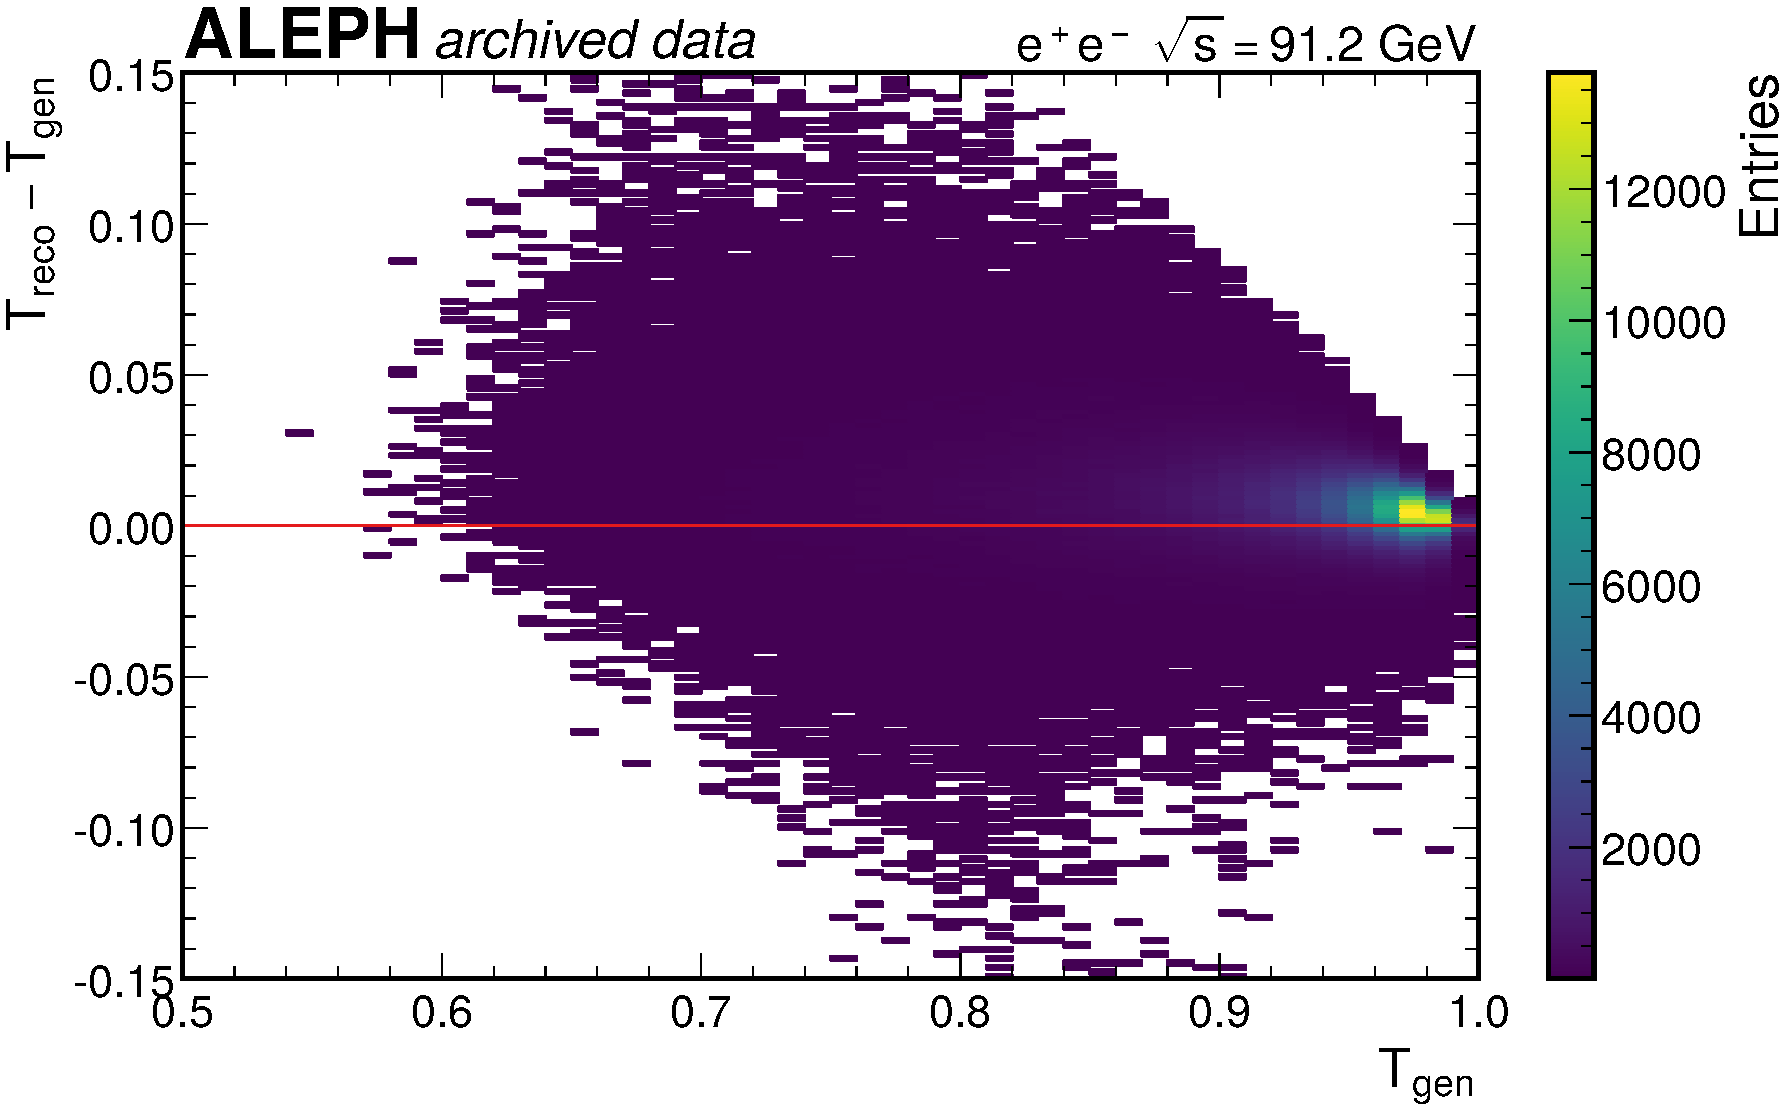
\includegraphics[width=0.85\textwidth]{figures/thrust_resolution_2d.pdf}
\caption{Thrust resolution $(T_{\mathrm{reco}}-T_{\mathrm{gen}})$ versus $T_{\mathrm{gen}}$ for matched MC event pairs.}
\label{fig:thrust_resolution_2d}
\end{figure}

\subsection{Unfolding setup and regularization choice}

Detector correction is performed with the IBU method of D'Agostini~\cite{DAgostini:1994zf,dagostini2010improvediterativebayesianunfolding}, as implemented in RooUnfold~\cite{Adye:2011gm},
\begin{equation}
U_j^{(n+1)} = \frac{1}{\epsilon_j}\sum_i M_i\,\frac{R_{ij}\,\pi_j^{(n)}}{\sum_k R_{ik}\,\pi_k^{(n)}},
\end{equation}
where $M_i$ is the measured detector-level spectrum, $R_{ij}$ is the response, and $\pi_j^{(n)}$ is the iteration prior. The prior for the first iteration is taken as the generator-level MC truth distribution $\pi_j^{(0)} = N_{\mathrm{gen}}(j)$, the standard RooUnfold default. This choice initializes the unfolding close to the expected truth shape and avoids any flat-prior amplification of high-frequency fluctuations in the first iteration. The response matrix is filled with MC events that pass the detector-level selection and the corresponding generator-level event as shown in Figure~\ref{fig:response_matrices_nominal}. A selected event whose reconstructed thrust falls outside the unfolding range enters instead through RooUnfold's miss term, which supplies the efficiency factor $1/\epsilon_j$ appearing below.

\begin{figure}[ht!]
\centering
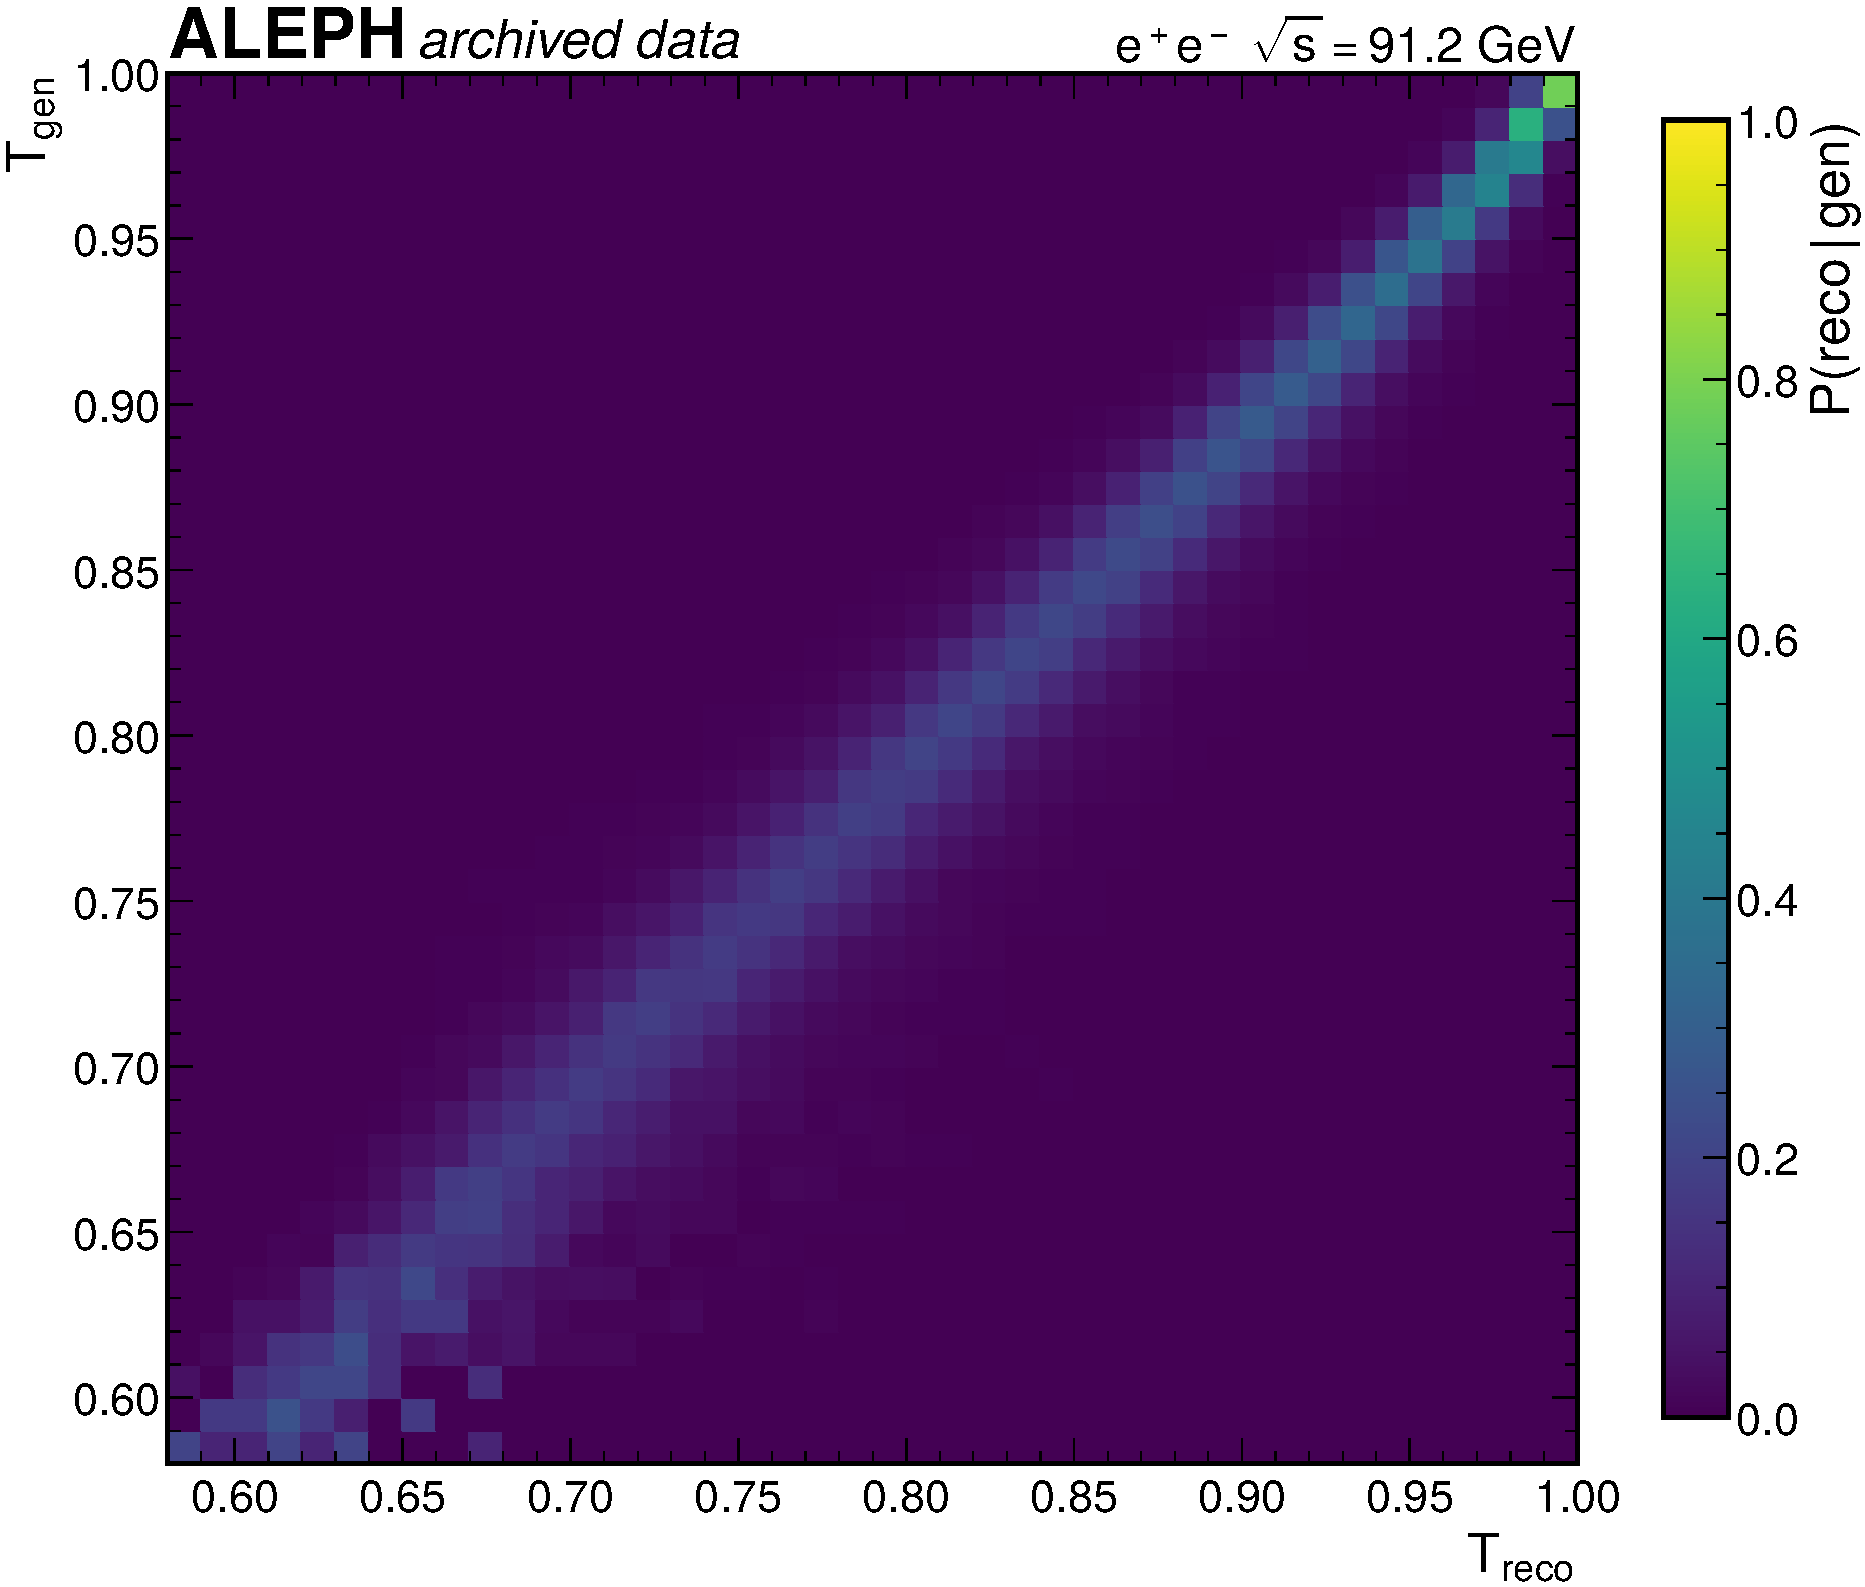
\includegraphics[width=0.85\textwidth]{figures/matrix_response_probability.pdf}
\caption{Nominal response probability matrix for thrust.}
\label{fig:response_matrices_nominal}
\end{figure}

The IBU regularization term for the number of iterations is kept at a nominal value of $N_{\mathrm{iter}}=5$ as found by previous studies~\cite{Badea:2019vey}, with $N_{\mathrm{iter}}=4$ and $6$ propagated as unfolding-regularization systematic branches.
The iteration-choice diagnostics, including refolded spectra at $N=4,5,6,10,100$ compared with detector-level data, confirm that the closure-shape $\chi^2/\mathrm{ndf}$ is stable for $N_{\mathrm{iter}}\in\{4,5,6\}$. The spread in the unfolded thrust spectrum across this range is below $1\%$ in 37 of the 42 reported bins (median $0.3\%$), rising to at most $6.6\%$ near the two-jet edge ($T\lesssim0.62$) where the steeply falling spectrum amplifies regularization sensitivity.

The response matrix has a diagonal fraction of $f_{\mathrm{diag}}=0.33$, meaning approximately two-thirds of events migrate out of their generated thrust bin at reconstruction level. This level of bin-to-bin migration is expected for thrust at ALEPH given the finite charged-particle momentum resolution and the sensitivity of thrust to soft particles near the event boundary. It implies that the unfolding correction is non-trivial and that the choice of regularization strength meaningfully affects the result. This also motivates the need to measure the final bin-by-bin correlation to assess the overall statistical strength.

The miss term, the generator-level events with no matched reconstructed counterpart, is
shown in Fig.~\ref{fig:miss_term_efficiency}. These are events that fail the reco-level hadronic event selection despite being generated within the fiducial volume. The miss rate is concentrated at low thrust ($T\lesssim0.7$) and in events with low charged multiplicity, consistent with the hadronic event selection removing poorly reconstructed events. RooUnfold accounts for miss events via \texttt{response.Miss($x_{\mathrm{gen}}$)}, which corrects the unfolded spectrum for this acceptance effect.

\begin{figure}[ht!]
\centering
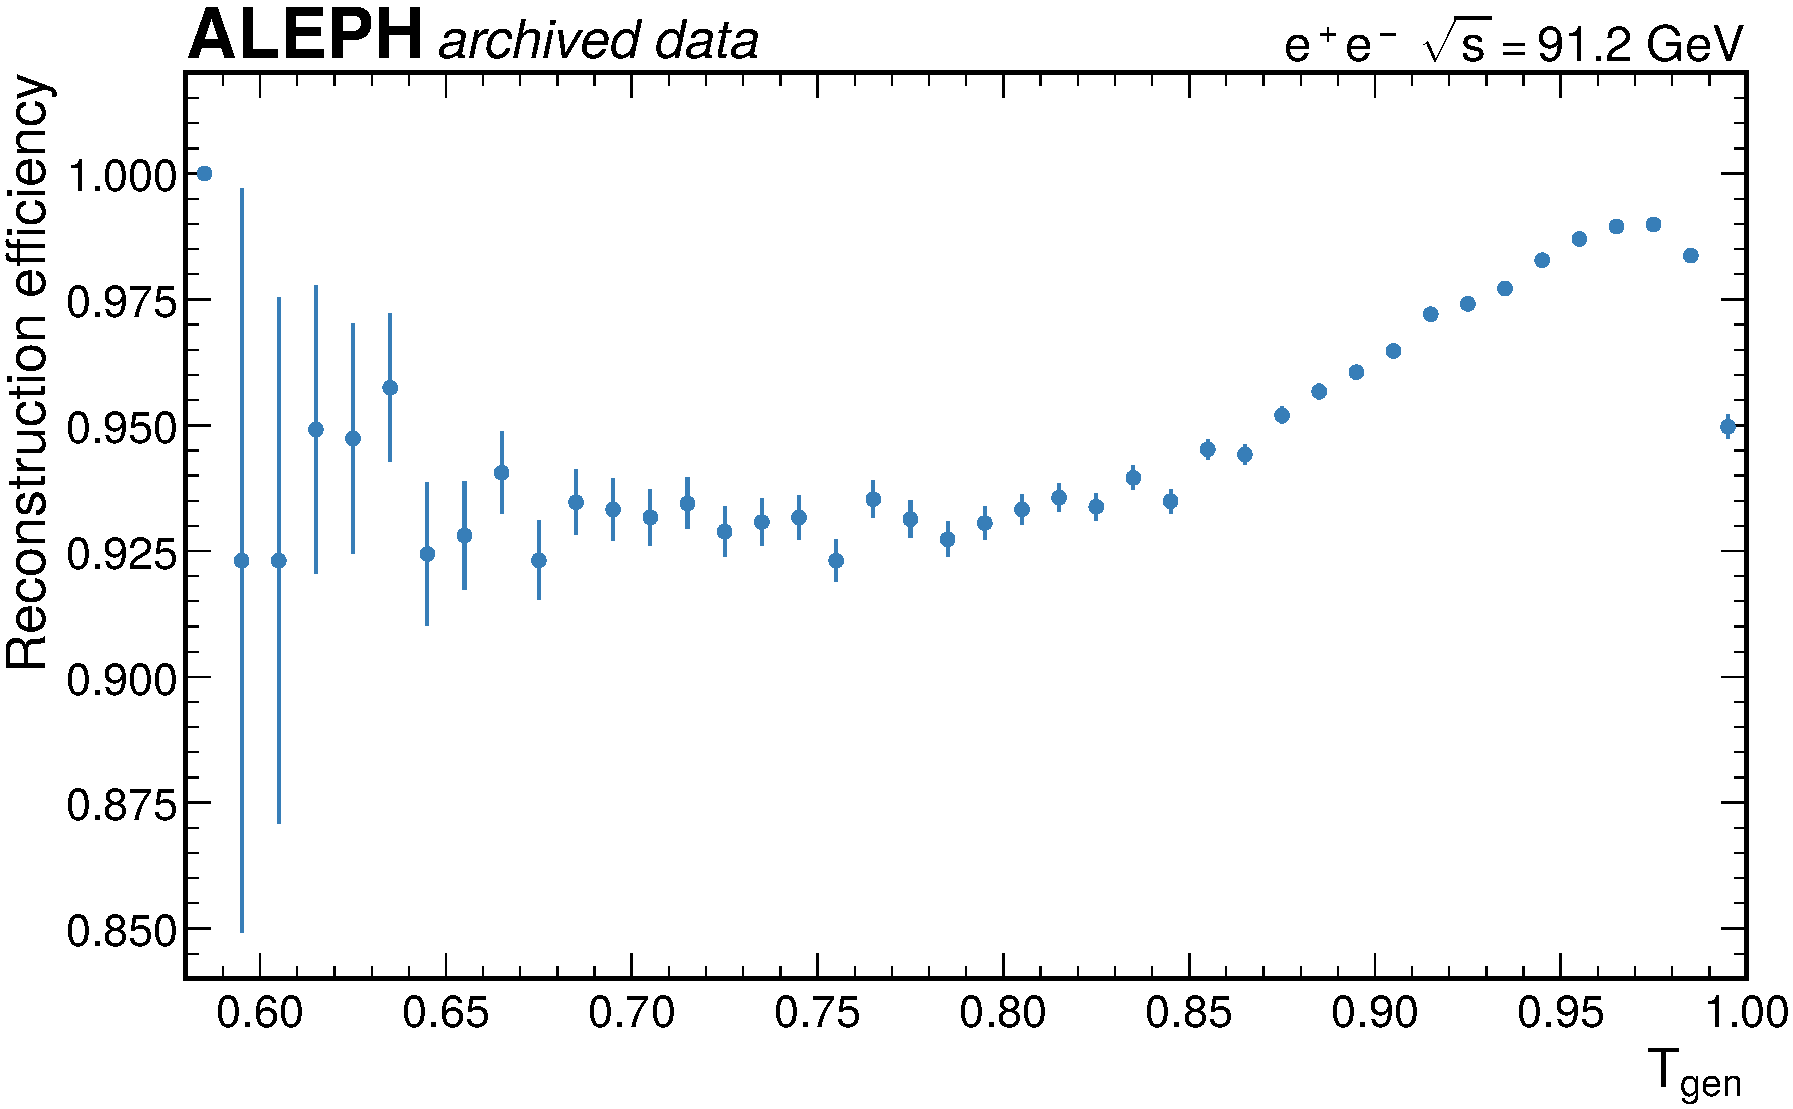
\includegraphics[width=0.49\textwidth]{figures/miss_term_efficiency.pdf}
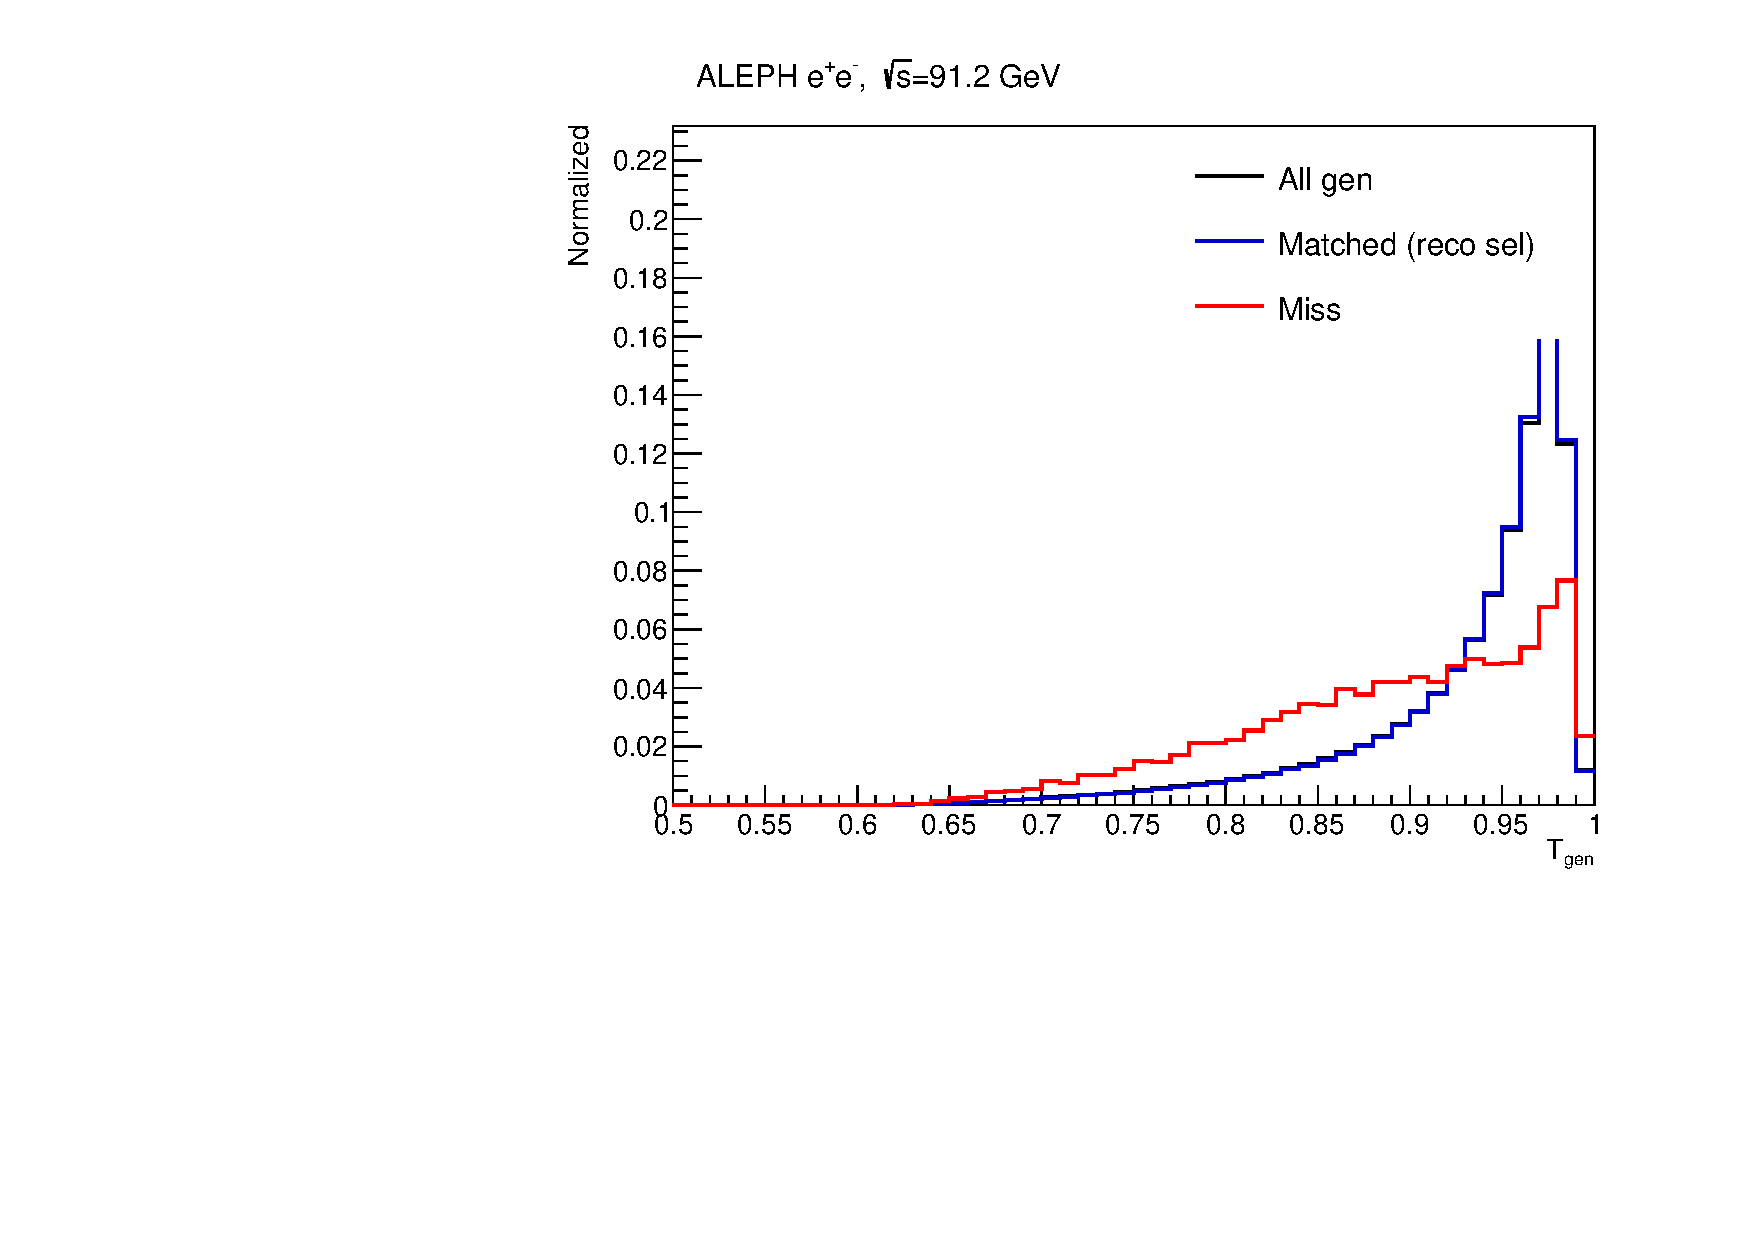
\includegraphics[width=0.49\textwidth]{figures/miss_term_thrust.pdf}
\caption{Left: reco efficiency (matched/all gen) as a function of $T_{\mathrm{gen}}$,
with binomial uncertainties. Right: thrust distributions for all gen, matched, and miss
events (normalized to unit area). Miss events are concentrated at low thrust and low
multiplicity, consistent with events failing the hadronic event selection.}
\label{fig:miss_term_efficiency}
\end{figure}

\subsection{Hadronic and QED ISR correction}
\label{sec:corrections_and_cov}

After unfolding, two multiplicative corrections are applied. A correction for the hadronic event-selection,
\begin{equation}
C_{\mathrm{had}}(j) = \frac{N_{\mathrm{genBefore}}(j)}{N_{\mathrm{gen}}(j)},
\end{equation}
accounts for the efficiency of the selection at the generator level. The correction factor is derived from the archived \textsc{Pythia}~6 sample~\cite{Sjostrand:2000wi} and is applied so that the final spectrum restores the yield lost by the hadronic selection.

Then a correction for electromagnetic (QED) initial-state radiation (ISR) is applied,
\begin{equation}
C_{\mathrm{ISR}}(j) = \frac{N^{\mathrm{gen}}_{\mathrm{no\,ISR}}(j)}{N^{\mathrm{gen}}_{\mathrm{ISR}}(j)}.
\end{equation}
This factor is applied to enable comparisons with state-of-the-art theory calculations which do not include QED ISR. The correction is derived from standalone \textsc{Pythia}~8.317 samples generated with ISR switched off and on~\cite{Bierlich:2022pfr}. \textsc{Pythia}~8.317 is chosen here for simplicity; a higher-order generator such as \textsc{KKMCee}~5.00.02 would be preferred for a full thrust measurement~\cite{Jadach:2022mbe}. The ratio histograms are pre-computed once into a cache file and applied identically to the nominal and all systematic variation branches, so that the ISR correction cancels in the systematic shifts and its residual uncertainty (from finite MC statistics on the ratio) is propagated as a separate component $\Delta_{\mathrm{ISR}}$ (Sec.~\ref{sec:isr_uncertainty}).

For the nominal result, the data statistical covariance is computed by RooUnfold using analytical error propagation (\texttt{RooUnfold::kCovariance}), which propagates Poisson uncertainties in the measured data through the IBU iteration chain without toy MC sampling. The response matrix's own finite statistics are not included by that call and are propagated separately by a Poisson bootstrap over the simulated events, as described in Sec.~\ref{sec:stat_uncertainty}. The resulting covariance matrices are read from the unfolding output and transformed to the normalized differential-thrust basis used in this work. Non-statistical component covariances are built with a configurable model, and all covariance products are exported over the reported bins.
